\documentclass[12pt,a4paper]{article}
\usepackage{vntex} % Tiếng Việt
\usepackage{graphicx} % Chèn hình ảnh
\usepackage{listings} % Thêm gói listings để chèn code
\usepackage{xcolor} % Màu cho code
\usepackage{changepage} % Thay đổi lề

\lstset{
    language=R,
    basicstyle=\footnotesize\ttfamily,
    numbers=none,
    numberstyle=\tiny\color{gray},
    stepnumber=1,
    numbersep=0.01pt,
    tabsize=2,
    breaklines=true,
    breakatwhitespace=false,
    xleftmargin=0cm, % for line numbers
    framexleftmargin=0cm, % for code frame
    keywordstyle=\color{blue},
    commentstyle=\color{green},
    stringstyle=\color{orange},
    frame=single,
    rulecolor=\color{black},
    basicstyle=\ttfamily,
}
% Thiết lập bảng
\usepackage{array}
\usepackage{tabularx}
\usepackage{longtable} % Tạo bảng qua nhiều trang
\usepackage{cellspace}
\usepackage{bm} % Chữ in đậm trong công thức toán 
\usepackage{a4wide,amssymb,epsfig,latexsym,multicol,array,hhline,fancyhdr}
\usepackage{tikz}
\usepackage{color}
\usepackage{subcaption}
\usepackage{framed}
\usepackage{float} % Để chèn hình ảnh vào đúng vị trí
\usepackage{fancyvrb} %Đưa dữ liệu dạng nguyên thủy vào
\usepackage{amsmath} % Công thức toán
% Thiết lập kích thước
\usepackage{geometry}
\geometry{
    left=3cm,
    right=2cm,
    top=2.5cm,
    bottom=2.5cm,
}
\usepackage{hyperref} %Chèn link
\hypersetup{urlcolor=black,linkcolor=black,citecolor=black,colorlinks=true} % Màu cho các đường nét
\everymath{\color{black}}
\setlength{\headheight}{40pt}
\pagestyle{fancy}


%Header
\fancyhead{} % clear all header fields
\fancyhead[L]{
 \begin{tabular}{rl}
    \begin{picture}(25,15)(0,0)
    \put(0,-8){
\includegraphics[width=12mm, height=12mm]{pictures/hcmut.png}}
    %\put(0,-8){\epsfig{width=10mm,figure=hcmut.eps}}
   \end{picture}&
	%
\includegraphics[width=8mm, height=8mm]{hcmut.png} & %
	\begin{tabular}{l}
		\textbf{\bf \ttfamily Trường Đại Học Bách Khoa - ĐHQG TP.Hồ Chí Minh}\\
		\textbf{\bf \ttfamily Khoa Cơ Khí - Bộ môn Cơ Điện Tử}
	\end{tabular} 	
 \end{tabular}
}
\fancyhead[R]{
	{\tiny \bf \quad} % Khoảng trắng nhỏ trong header bên phải
}

%Footer
\fancyfoot{} % clear all footer fields
\fancyfoot[L]{\scriptsize \ttfamily Trang bị điện - điện tử trong máy công nghiệp}
\fancyfoot[R]{\scriptsize \ttfamily Trang {\thepage}/13}
\renewcommand{\headrulewidth}{0.3pt}
\renewcommand{\footrulewidth}{0.3pt}

\begin{document}
    \begin{titlepage}   
    \begin{center}
        \vspace*{-2cm} 
        \large
        \textbf{ĐẠI HỌC QUỐC GIA THÀNH PHỐ HỒ CHÍ MINH \\
        TRƯỜNG ĐẠI HỌC BÁCH KHOA\\
        KHOA CƠ KHÍ\\
        BỘ MÔN CƠ ĐIỆN TỬ}\\
        
\includegraphics[width=70mm, height=70mm]{./pictures/hcmut.png} \\
        \rule{\linewidth}{0.5mm}\\
        \vspace{0.8cm}
        \Large
        \textbf{TRANG BỊ ĐIỆN - ĐIỆN TỬ TRONG MÁY CÔNG NGHIỆP}\\
        \vspace*{0.5cm}
        \Huge
        \textbf{EXERCISE 1}\\
        \vspace{0.5cm}
        \rule{\linewidth}{0.5mm}\\
        \vspace{0.8cm}
        \vspace{1cm}
        \large
        GVHD: TS. LÊ ĐỨC HẠNH\\
        \vspace{0.5cm}
        DANH SÁCH THÀNH VIÊN:\\[0.3cm]
        \begin{tabular}{|>{\centering\arraybackslash}m{1cm}|>{\centering\arraybackslash}m{7cm}|>{\centering\arraybackslash}m{5cm}|}
            \hline
            \textbf{STT} & \textbf{Họ và tên} & \textbf{MSSV} \\
            \hline
            1 & Võ Hữu Dư & 2210604 \\
            \hline
            2 & Dương Quang Duy & 2210497 \\
            \hline
            3 & Trần Quang Đạo & 2210647 \\
            \hline
        \end{tabular}
    \end{center}
        
    \vfill
    \large
    \begin{center}
        TP.HCM, \today
    \end{center}
\end{titlepage}

	\tableofcontents
	\newpage
	\section{Thiết kế mạch khuếch đại dùng opamp tạo sóng ngõ ra và kiểm tra lại bằng proteus}	
		\subsection{Câu a.$\mathbf{v_o = 0.5 \cdot v_1 - 3 \cdot v_2 + 4 \cdot v_3}$}
			\subsubsection{Tính toán mạch khuếch đại dùng opamp}
				\begin{figure}[H]
					\centering
					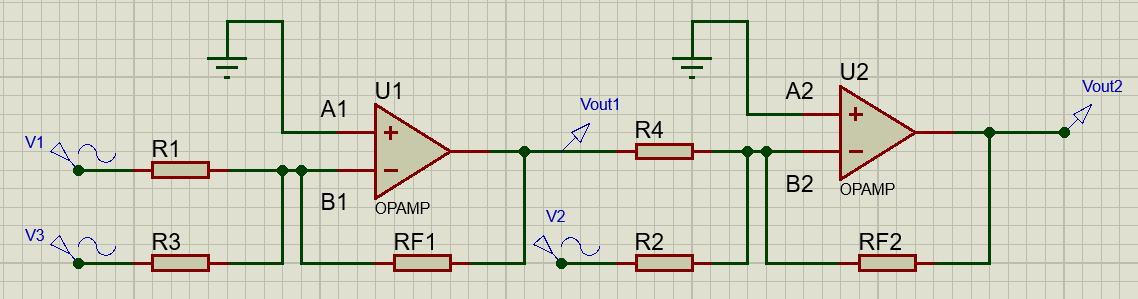
\includegraphics[width=0.7\textwidth]{pictures/topic1_a.png}
					\caption{Mạch khuếch đại dùng opamp}					
					\label{fig:circuit_simulation}
				\end{figure}
				\hspace*{0.6cm}\textbf{Giả sử KĐTT là lý tưởng}
				\[
				\Rightarrow
				\begin{cases}
					I^+ = I^- = 0\\
					V_{A1} = V_{B1} = V_{A2} = V_{B2} = 0\\
				\end{cases}
				\]
				\hspace*{0.6cm}Dòng điện đầu ra Opamp thứ nhất là:
				\begin{align}
					V_{out1} = -\frac{R_{F1}}{R_1} \cdot V_1 - \frac{R_{F1}}{R_3} \cdot V_3 
				\end{align}
				\hspace*{0.6cm}Dòng điện đầu ra Opamp thứ hai là:
				\begin{align}
					V_{out2} = -\frac{R_{F2}}{R_4} \cdot V_{out1} - \frac{R_{F2}}{R_2} \cdot V_2
				\end{align}
				\hspace*{0.6cm}Thế (1) vào (2) ta được: 
				\begin{align*}
					V_{out2} &= -\frac{R_{F2}}{R_4} \cdot \left(-\frac{R_{F1}}{R_1} \cdot V_1 - \frac{R_{F1}}{R_3} \cdot V_3\right) - \frac{R_{F2}}{R_2} \cdot V_2 \\
							&= \frac{R_{F1} \cdot R_{F2}}{R_1 \cdot R_4} \cdot V_1 + \frac{R_{F1} \cdot R_{F2}}{R_3 \cdot R_4} \cdot V_3 - \frac{R_{F2}}{R_2} \cdot V_2
				\end{align*}
				\hspace*{0.6cm}Theo đề bài ta có: $V_{out2} = 0.5 \cdot V_1 - 3 \cdot V_2 + 4 \cdot V_3$
				\[
				\Rightarrow
				\begin{cases}
					\frac{R_{F1} \cdot R_{F2}}{R_1 \cdot R_4} = 0.5\\
					\frac{R_{F1} \cdot R_{F2}}{R_3 \cdot R_4} = 4\\
					\frac{R_{F2}}{R_2} = 3
				\end{cases}
				\]
				\hspace*{0.6cm}Chọn $R_{2} = 50k\Omega$ $\Rightarrow$ $R_{F2} = 150k\Omega$.\\
				\hspace*{0.6cm}Chọn $R_{1} = 200k\Omega$, $R_{4} = 150k\Omega$ $\Rightarrow$ $R_{F1} = 100k\Omega$ $\Rightarrow$ $R_3 = 25k\Omega$.\\
			\newpage
			\subsubsection{Kiểm tra lại bằng proteus}
				\begin{itemize}
					\item Sử dụng Proteus để mô phỏng mạch như hình \ref{fig:circuit_simulation}
					\item Sử dụng các linh kiện: Opamp, Resistor, Voltage Source Sine, Ground
					\item Gán các giá trị điện trở như giá trị tính được ở trên.
					\item Cho các giá trị điện áp đầu vào $V_1 = 1V$, $V_2 = 2V$, $V_3 = 3V$.
					\item Kết quả mô phỏng được như hình \ref{fig:result_simulation}
					\begin{figure}[H]
						\centering
						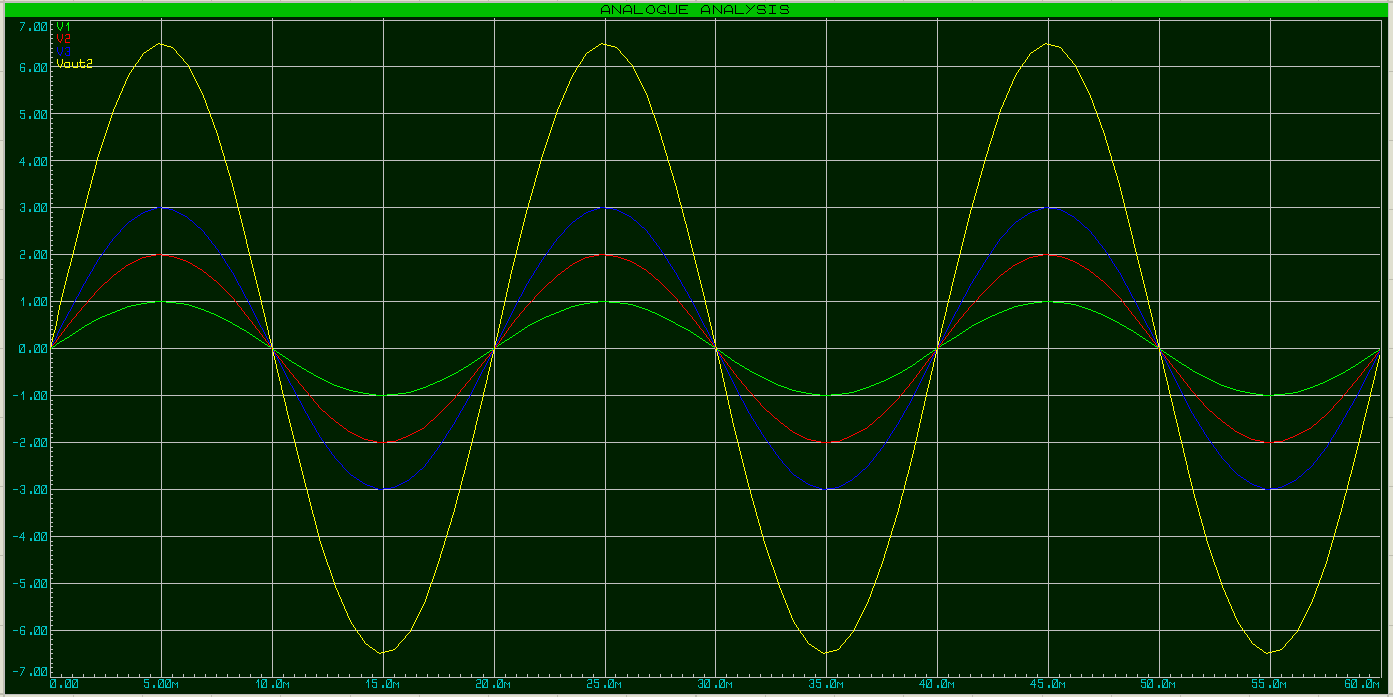
\includegraphics[width=0.7\textwidth]{pictures/result1_a.png}
						\caption{Mạch khuếch đại dùng opamp}					
						\label{fig:result_simulation}
					\end{figure}
					\item Ta thấy giá trị điện áp đầu ra $V_{out} = 0.5V_1 - 3V_2 + 4V_3 = 0.5 \cdot 1 - 3 \cdot 2 + 4 \cdot 3 = 6.5V$ giống với đồ thị analog $\Rightarrow$ Kết quả mô phỏng proteus giống với giá trị tính toán.
				\end{itemize}
		\subsection{Câu b.$\mathbf{v_o = 0.5 \cdot v_1 - 3 \cdot v_2 + 4 \cdot v_3}$}
\end{document}